\chapter{Generalised Ensemble Methods}
{\color {red} 
\section{Introduction@@WILL BE REMOVED}}
Protein-protein or protein-ligand complex is stabilized or destabilized by a variety of factors, and atomic-detailed information on the intermolecular interactions provides a crucial key to understand the complex formation in a microscopic points of view, and this information may support drug discovery. Biomolecular complex formation is a process where the biomolecules associate starting from the dissociated state, and finally a biologically meaningful complex is formed. The experimentally determined complex structure may be the lowest free-energy state, which is equivalent to the thermodynamically most stable complex. However, recent study also has shown that various complex forms other than the most stable complex one are generated in the binding process, such as encounter complexes [1], metastable complexes, or fuzzy complexes [2], and these multiple complex forms may play a biologically/biophysically meaningful role. Those complexes may be formed transiently with weak interactions. Therefore, we propose a question: Is there any method that can provide atomistic information for the multiple complexes? In other words, is there any method that can assign free energies (i.e., stabilities) to the multiple complexes? 

It is generally difficult to determine temporal complex structures, in which the biomolecules are weakly interacting. Then an all-atom computer simulation such as molecular dynamics (MD) is a useful technique to quantify those complex structures because the all-atom simulations can trace biomolecular motions at an atomic resolution at each moment of the complex formation. Figure \ref{fig:u_b_states_pic} schematically presents the processes of complex formation, where semi-stable structural clusters together with the most stable one are illustrated. Imagine a simulation, during which association and dissociation of molecules take place. The number of simulation snapshots assigned to a cluster relates to its stability (i.e., free energy): The more the snapshots in a cluster there are, the lower the free energy assigned to the cluster. Frequency of transitions from a cluster to another relates to the rate constant for the conformational change. Therefore, the simulation trajectory yields a diagram such as Figure \ref{fig:u_b_states_pic}.
\begin{figure}
  \centering
  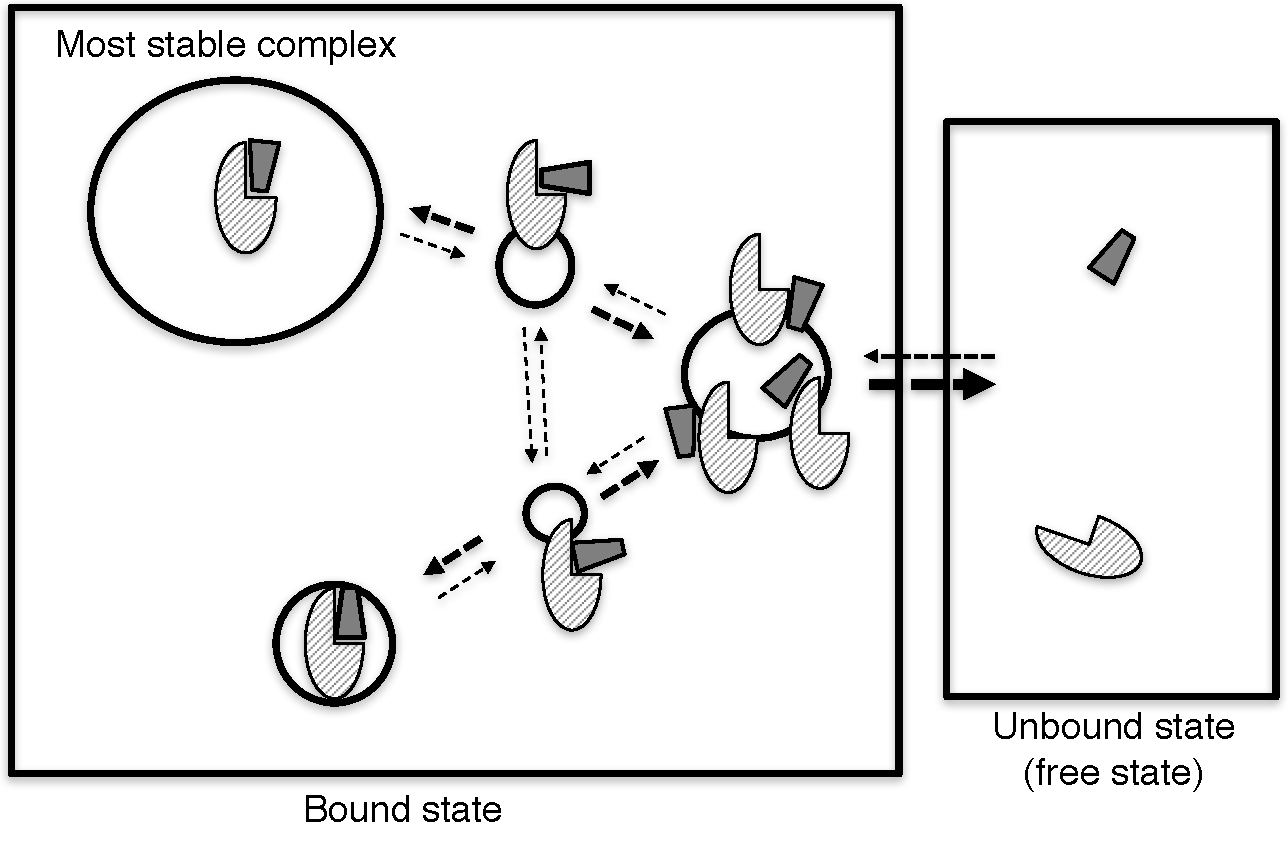
\includegraphics[width=10cm]{../enhance_rev/figures/u_b_states_pic.pdf}
  \caption{\label{fig:u_b_states_pic}}
\end{figure}

A quantitatively evaluated diagram is called a free-energy landscape and provides key information to discuss the complex formation in detail. Because conventional sampling methods have difficulty in obtaining an ensemble of snapshots enough to generate the free-energy landscape, several powerful computation methods have been developed. One way to approach the free-energy landscape is to use a powerful computer such as ANTON [3,4] or MDGRAPE [5] to perform a long time simulation. The second way is to integrate many simulation trajectories, where the trajectories generate a wide conformational distribution [6] or rate constant among conformational clusters [7,8], although each trajectory may cover only a small fraction of the whole conformational space. The third way is to use a generalized ensemble method [9,10]. In this review, we focus on various generalized ensemble methods that have been applied or are applicable to biomolecular binding with an atomistic resolution in an explicit solvent to obtain the free-energy landscape. Table 1 lists the generalized ensemble methods that are introduced in this review. We note that these methods are also applicable to large molecular conformational changes such as protein folding or intra-molecular conformational transitions by changing the computation object. In fact, many of the methods have been applied to folding in the referred papers.

In computational biophysics, development of an effective conformational sampling method has been one of the central subjects. When force field parameters are assigned to constituent atoms of the system (protein(s), ligand(s), and solvents), the potential energy is computable to the protein system. In this paper, potential energy is called “energy” simply. Different conformations of the system have different energy. Therefore, an energy surface (Figure \ref{fig:ene_landscape.pdf}a) can be constructed for the system in theory. Problems are: the energy surface of the protein system has a large number of energy basins surrounded by energy barriers, and some of conformational transitions among the basins are very slow processes. These difficulties arise as a result of the following factors: (i) The original conformational space is 3n-dimensional for a system consisting of n atoms, and n is usually large. (ii) Various types of interactions act among the constituent atoms. (iii) Usually there is no structural symmetry in the system. (iv) Motions of an atom are influenced strongly by the surrounding atoms because the atoms are densely packed. 
\begin{figure}
  \centering
  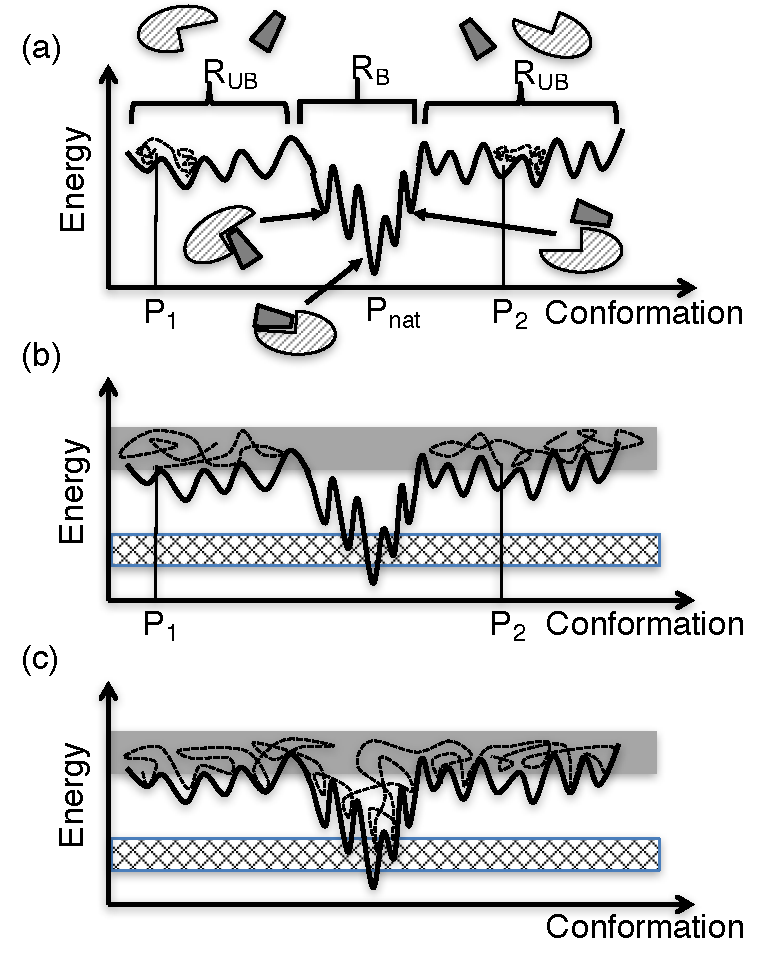
\includegraphics[width=10cm]{../enhance_rev/figures/ene_landscape.pdf}
  \caption{\label{fig:ene_landscape.pdf} Schematic representation of energy surface and simulation trajectories.
$X$- and $y$-axes represent conformation and energy for a two-molecular system,
respectively. Black curved line represents the energy surface, where energy minima and energy barriers distribute. Although the conformation of the system is defined originally in a high-dimensional space, the space shown in this figure is one-dimensional (i.e., $x$-axis). Molecular structures are also shown schematically. $\rm R_{\rm UB}$ is a region where unbound or slightly contacting molecules are distributed, and $\rm R_{\rm B}$ a region where various complex forms distribute. Although $\rm R_{\rm UB}$  is divided into two in this figure, they may be connected in the original high-dimensional space. (a) Broken lines represent simulation trajectories at room temperature starting from conformations at $\rm P_1$ and $\rm P_2$, which are far from the native complex structure ($\rm P_{\rm nat}$). The conformation moves slowly in the space because energy barriers interfere the motion. (b) Simulation trajectories (broken lines) at high temperature. The trajectories fluctuate in a high-energy range (shaded energy range), which involves $\rm R_{\rm UB}$, and the room-temperature range (checked range) is not sampled. Volume of $\rm R_{\rm B}$ is considerably narrower than that of $\rm R_{\rm UB}$ in the original high-dimensional space. (c) Trajectory from multicanonical simulation, which sample evenly the high and low energy ranges.}
\end{figure}

When one performs a molecular simulation at room temperature (denoted as $T_{\rm room}$ ), the conformation of the protein is usually trapped in energy basins near the initial conformation of the simulation (Figure \ref{fig:ene_landscape.pdf}a). Note that majority of proteins exert their biological functions at the room temperature, and then many biological experiments have been performed at this temperature. Then, to sample a wide conformational area with overcoming energy barriers and reach the native complex structure (i.e., experimentally determined complex structure at $T_{\rm room}$), a long simulation is required when the simulation starts from a dissociated conformation. A simple method to sample various conformations without being trapped is a high-temperature simulation (Figure \ref{fig:ene_landscape.pdf}b). This method, however, generates conformations accessible only at the high temperature. Inversely, when the high-temperature simulation starts from the native complex structure, this complex dissociates eventually, and the transition probability that the dissociated molecules rebind again to the native complex is negligibly small. A requirement imposed on the sampling method is that the resulted ensemble should consist of conformations probable at $T_{\rm room}$ in equilibrium (conformations in the checked energy range in Figure \ref{fig:ene_landscape.pdf}b) even when the simulation starts from a dissociated conformation. We denote this ensemble as $Q(T_{\rm room})$. The free energy landscape is derived from $Q(T_{\rm room})$. \textcolor{red}{@@@No (c)???}

The high-dimensional space to express the protein conformation is beyond our comprehension. Then, contraction of the high-dimensional space into a low-dimensional space is essential. Some parameters, such as relative molecular orientation of one molecule to the other, separation distance between two molecules, or root mean square deviation from a reference complex structure, are useful to construct the low-dimensional space for viewing the conformational distribution. Suppose that two parameters, denoted as  $s_1$ and$s_2$ , are selected for the coordinate axes of the contracted space (here it is a two-dimensional (2D) space). Then a set of parameters $[s_1, s_2]$ is calculated for all of the conformations stored in $Q(T_{\rm room})$, and a probability distribution function $P_{\rm cano}(s_1, s_2, T_{\rm room})$ is computed. A “potential of mean force (PMF)”, $F(s_1, s_2, T_{\rm room})$ , is formally defined as:
\begin{equation}
F(s_1, s_2, T_{\rm room})=-RT \ln [P_{\rm cano}(s_1, s_2, T_{\rm room})],
\label{eq:pmf}
\end{equation}
where $R$ is the gas constant. Equation \ref{eq:pmf} shows that a low PMF is assigned to a high-probability position. Note that high-probability regions in the conformational space are more stable thermodynamically than low-probability regions. In other words, the low-PMF regions are thermodynamically stable. Therefore, PMF is regarded as a free-energy landscape. The low-PMF regions are called “free-energy basins”, and the parameters $s_1$ and $s_2$ are called “reaction coordinates”. Figure \ref{fig:pmf_pic.pdf} illustrates the relation between $P_{\rm cano}$ and $F$ in one-dimensional case. In a general case, $P_{\rm cano}$ is converted as:
\begin{equation}
F(s_1,s_2,s_3,..,s_n, T_{\rm room})=-RT_{\rm room} \ln [P_{\rm cano}(s_1,s_2,s_3,..,s_n, T_{\rm room})],
\label{eq:pmf_gene}
\end{equation}
where both $P_{\rm cano}$ and $F$  are expressed by $n$ parameters.
\begin{figure}
  \centering
  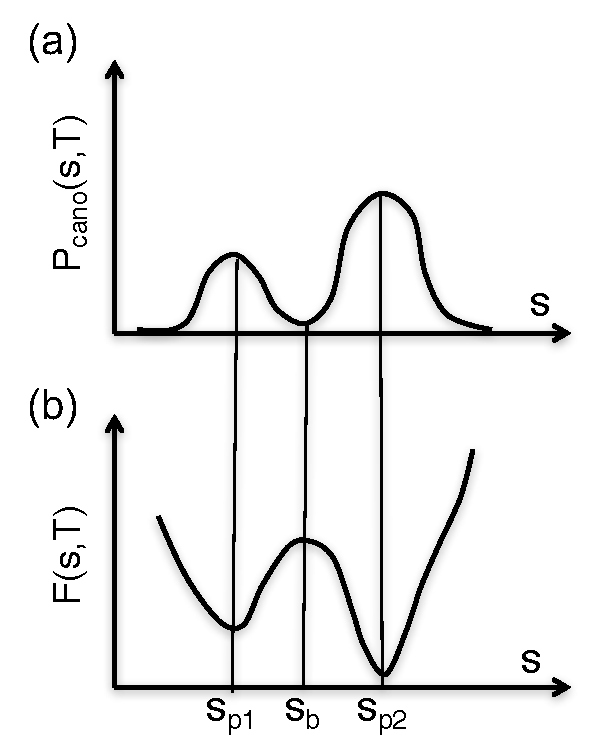
\includegraphics[width=10cm]{../enhance_rev/figures/pmf_pic.pdf}
  \caption{\label{fig:pmf_pic.pdf} Conversion of distribution function to PMF in one-dimensional case. One-dimensional parameter is denoted as $s$. (a) Distribution $P(s,T)$, and (b) PMF: $F(s,T)=-RT \ln[P(s,T)]$. High probability is assigned to $s_{\rm p1}$ and $s_{\rm p2}$, where $F(s,T)$ is low. Contrarily, the low-probability is assigned to $s_{\rm b}$, where $F(s,T)$ is high.}
\end{figure}

\section{Umbrella Sampling}
As an enhanced sampling method, we first introduce umbrella sampling [11,12]. In this method, an appropriate reaction coordinate $p$ is set in advance so that the variation of $p$ reflects well the change of complex form. Figure \ref{fig:us_picture.pdf}a shows schematically the $p$-axis, which connects the unbound ($p_u$) and the native-complex structures ($p_n$). The umbrella sampling method introduces bias functions called “umbrella potential functions” along the $p$-axis. A bias potential set at a bias center (one of the filled or open circles in Figure \ref{fig:us_picture.pdf}a) affects the conformation to be confined within a narrow region around the bias center during a simulation. Then, performing individual simulations at different bias centers at temperature $T_{\rm room}$, one can obtain a number of biased distribution functions (Figure \ref{fig:us_picture.pdf}b). The purpose of the umbrella sampling is to obtain an entire distribution function $P_{\rm cano}(p, T_{\rm room})$ without the effects of the bias potentials in the full range $[p_u,p_n]$ of the $p$-axis. Then a reweighting technique is applied on each of the biased distributions, and non-biased fragments of the entire distribution (Figure \ref{fig:us_picture.pdf}c) are obtained. Finally, smooth connection of the fragments produces $P_{\rm cano}(p, T_{\rm room})$ (Figure \ref{fig:us_picture.pdf}d). This connection technique is called a "weighted histogram analysis" [13]. After the simulations, sampled snapshots are also reweighted and integrated into the conformational ensemble $Q(T_{\rm room})$. 
\begin{figure}
  \centering
  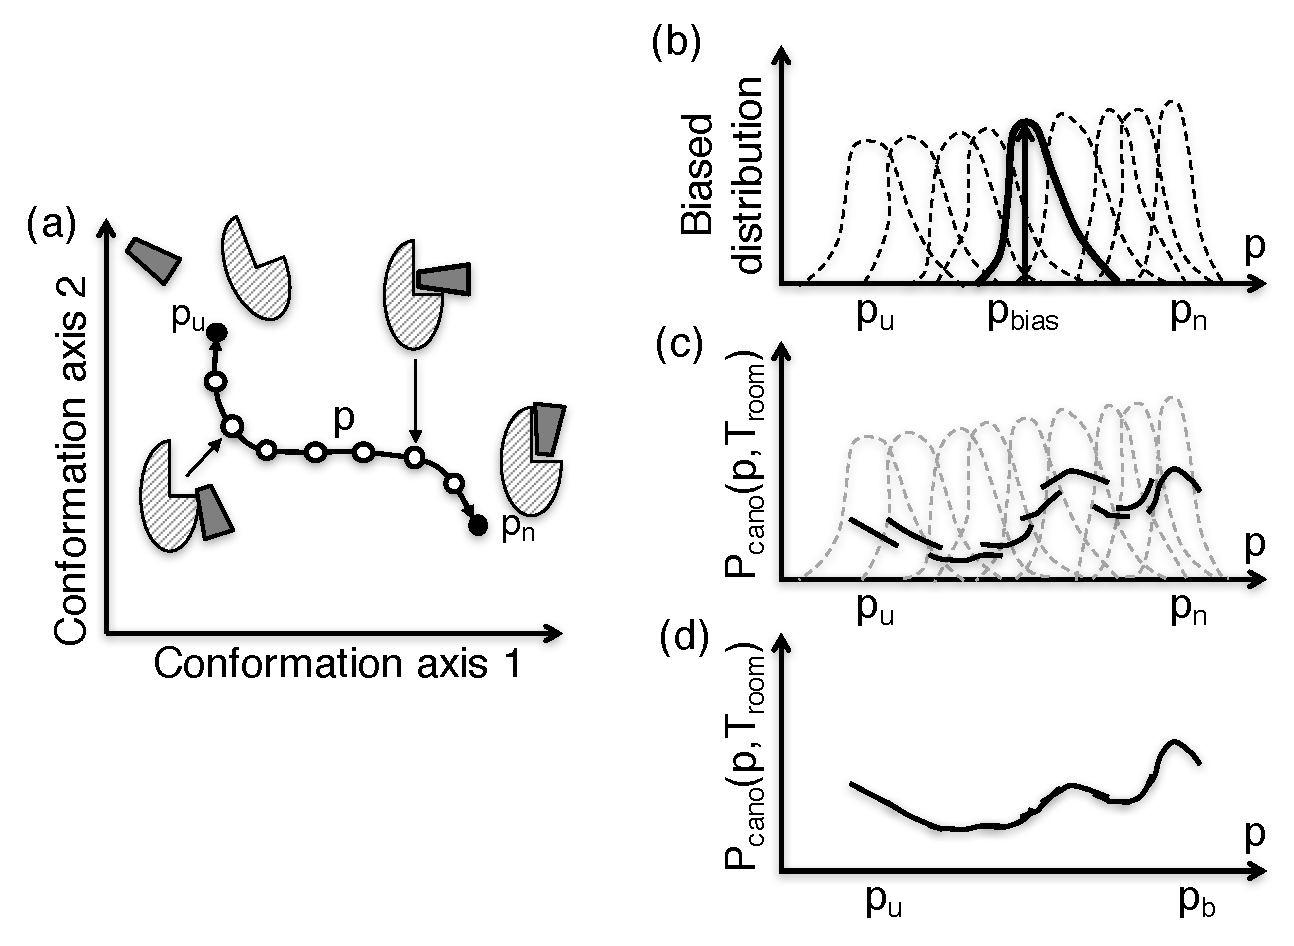
\includegraphics[width=10cm]{../enhance_rev/figures/us_picture.pdf}
  \caption{\label{fig:us_picture.pdf} Scheme for explaining umbrella sampling. (a) High-dimensional space is expressed here two-dimensionally ("conformational axis 1" and "conformational axis 2"), and reaction coordinate p is defined, for which the edges with filled circles labeled pu and pn correspond to unbound and native complex conformations, respectively. Open circles are intermediate conformations along the $p$-axis. (b) Biased distribution functions (broken and solid lines) obtained by individual simulations at different bias centers at temperature Troom . The solid line highlights a distribution around bias center pbias . (c) Solid lines are fragments of the full distribution function $P_{\rm cano}(p,T_{\rm room})$. Each fragment is computed only in well-sampled region of a biased distribution function in panel b.(d) $P_{\rm cano}(p,T_{\rm room})$ is obtained by smoothly connecting the fragments.}
\end{figure}

\section{Adaptive Umbrella Sampling}
“Adaptive umbrella sampling (AUS)” [14,15] also introduces a bias function. However, this bias function is not for restricting the conformation in a narrow range of the reaction–coordinate $p$. Contrarily, the bias assists the conformation to fluctuate in the range $[p_u, p_n]$ smoothly (Figure \ref{fig:dist_for_aus.pdf}a). In short, AUS is a method to enhance the conformational fluctuations along the reaction-coordinate. The bias potential $E_{\rm aus}$ is given as:
\begin{equation}
E_{\rm AUS} = E + RT_{\rm room} \ln [P_{\rm cano}(E,T_{\rm room})].
\label{eq:e_aus}
\end{equation}
Note that the second term of the right side of this equation is PMF (see Eqs. 1 and 2). An MD simulation at $T_{\rm room}$, where $E_{\rm AUS}$ is used for evaluation of inter-atomic forces ($force=-\nabla E_{\rm AUS}$), produces a flat distribution function  along the -axis (Figure \ref{fig:dist_for_aus.pdf}b) when the function  is accurate enough and the simulation is long enough: $P_{\rm AUS}(p,T_{\rm room}) \approx const$.
\begin{figure}
  \centering
  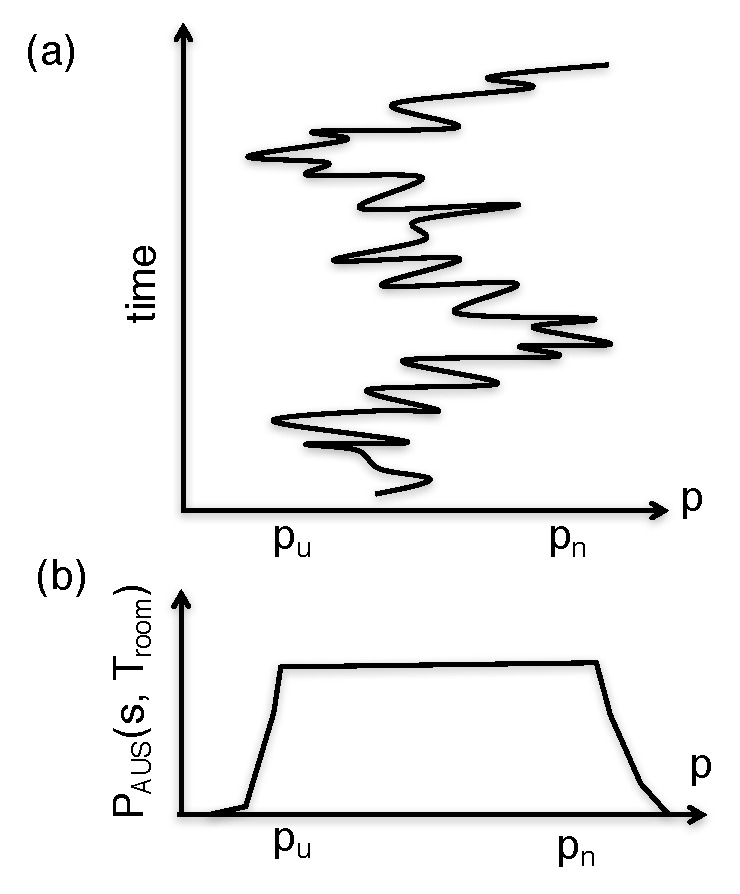
\includegraphics[width=10cm]{../enhance_rev/figures/dist_for_aus.pdf}
  \caption{\label{fig:dist_for_aus.pdf} Scheme for adaptive umbrella sampling (AUS). (a) The conformation fluctuates in range $[p_u, p_n]$ of reaction-coordinate axis $p$ with time. (b) Conformational distribution $P_{\rm AUS} (p ,T_{\rm room})$ resulted from AUS.}
\end{figure}

Note that the distribution function $P_{\rm cano}(E,T_{\rm room})$ is unknown in advance, and then, this function is refined iteratively through simulations [10]: After a simulation has been finished, $P_{\rm cano}(E,T_{\rm room})$ is updated from the simulation trajectory, and the next simulation is started using the updated function, and so on. Through the iterations, $P_{\rm AUS}(p,T_{\rm room})$ is flattened more and more, and when $P_{\rm AUS}(p,T_{\rm room})$ becomes flat enough, we judge that  is accurate enough. Finally, we perform a long simulation using the refined $P_{\rm cano}(E,T_{\rm room})$ and store snapshots. Then $Q(T_{\rm room})$ is generated where a thermal weight at $T_{\rm room}$ is assigned to each of the stored snapshots (reweighting).

\section{Metadynamics(Higo version)}
A method called “metadynamics” refines $P_{\rm cano}(E,T_{\rm room})$ within a simulation [16,17]. Thus, metadynamics is an iteration-free method and, thus, suitable for automation of simulation procedure [10]. Wang-Landau sampling [18], which enhances the conformational fluctuations along the energy axis as explained later, also refine a bias potential within a simulation.
\section{Metadynamics (Shinji version)}

\section{Multicanonical Sampling}
Multicanonical sampling was proposed originally to study statistical properties of a physical model, Potts model [19]. In this work, the Metropolis Monte-Carlo algorithm was carried out to explore the conformational space. Then, this method was applied to biological systems [20-23], and extended to an MD scheme where Newtonian equations were solved in the Cartesian coordinate space [24]. We denote this MD-based multicanonical method “McMD”. The adoption of the Cartesian coordinates makes the sampling applicable readily to a multi-polypeptide system in explicit solvent [25]. 

As with the adaptive umbrella sampling, multicanonical sampling introduces an energy bias function (multicanonical potential energy) as:
\begin{equation}
\label{eq:e_mc}
E_{\rm MC} = E + RT_{\rm room} \ln [P_{\rm cano}(E,T_{\rm room})],
\end{equation}
where $P_{\rm cano}(E,T_{\rm room})$ is the canonical energy distribution function at . An MD simulation using atomic forces of $force=-\nabla E_{\rm MC}$ at $T_{\rm room})$ produces a flat distribution function ($P_{\rm MC} \approx const$) along the energy axis when the function  is accurate enough and the simulation is long enough. Therefore, the multicanonical sampling enhances the fluctuations along the energy axis: When the system is in a high-energy range (the shaded range in Figure \ref{fig:ene_landscape.pdf}c), the conformation can overcome energy barriers, and when the system is in a low-energy range (the checked range in Figure \ref{fig:ene_landscape.pdf}c), which corresponds to the room-temperature range, the sampled conformations are accumulated into the ensemble $Q(T_{\rm room})$.

Recently, trajectory parallelization has been combined with McMD [6,26], and applied to a system consisting of a fragment taken from an intrinsically disorder protein and its partner protein in explicit solvent [27]. Furthermore, a virtual system, which has arbitral physical properties defined by a researcher, has been introduced to enhance sampling and coupled with the biomolecular system [28]. This procedure was named “virtual-system coupled multicanonical molecular dynamics (V-McMD)”. The V-McMD method was combined with the trajectory parallelization and applied to the p53 inter-domain linker, which is an intrinsically disordered region of p53 to regulate the p53–DNA interactions [29].

As well as the adaptive umbrella sampling, the distribution function $P_{\rm cano}(E,T_{\rm room})$ is unknown in advance. Then this function is determined iteratively: When the i-th simulation run has been finished, $P_{\rm cano}(E,T_{\rm room})$ is updated using a recurrent equation (see Ref. 10), $E_{\rm MC}$ is refined using Eq. \ref{eq:e_mc}, and the (i+1)-th run is performed. We call this procedure an “every-run” update method. As mentioned above, the Wang–Landau sampling method [18] updates $P_{\rm cano}(E,T_{\rm room})$ at every step of simulation. We call this updating method an “every-step” update method. A force-biased multicanonical MD [30] is a method in between the every-run and every-step update methods: A long simulation can be regarded as a succession of simulation intervals (blocks). After a block has been finished, $P_{\rm cano}(E,T_{\rm room})$ is updated using the data in this block, and the simulation for the next block is started using the updated $P_{\rm cano}(E,T_{\rm room})$. We call this method an “every-interval” update method. This method is also suitable for automating the simulation procedure.

\section{Simulated Annealing}
Not being a generalised ensemble method, simulated annealing methods, which has been applied to Monte Carlo and molecular dynamics simulations, can also search for energy minima in a potential energy surface of a physical system [ref]. 

The essential idea is the consideration of temperature of the system:
Increasing temperature of a physical system, the method makes a variety of configuration  accessible, and then it cools the system, thereby being able to search for an energy minimum. If we want to explore many energy minima, then SA simulations must be started with different initial configurations.

In general, it is said that the decrease speed of temperature should be slow in order to avoid becoming trapped in high potential energy regions and to explore thoroughly a potential surface {\color{red} [WHY THEY HAPPEN IF DO THAT?]}. However, {\color {red} FIXME there is no way to avoid the problems exactly.} Even in a rude cooling schedule, we may obtain a good result.

\section{Simulated Tempering}
Simulated tempering [31,32] is a method where temperature of the system changes as $T_1 \rightarrow T_2 \rightarrow T_3 \cdots$ during a simulation with satisfying the detailed balance condition at the temperature switching, and similar methods with the simulated tempering have been proposed [33-35]. In this method, temperature fluctuates covering a range from room to high temperatures. When the temperature is elevated, the system overcomes energy barriers. 

\section{Temperature Replica Exchange Method (Parallel Tempering)
{\color{red} (add figures to explain REMD)}
}
A method called “temperature replica exchange method (tREM)” [36,37] or “parallel tempering” [38] introduces multiple systems (replicas), whose chemical compositions are exactly the same one another, although the temperatures are different. These replicas evolve according to the Newtonian equations of motion (or Monte Carlo method) for a while, and occasionally exchange their temperatures imposing the detailed balance condition at the temperature exchange. Therefore, each replica experiences various temperatures during the time–evolution. Importantly, replicas overcome energy barriers when their temperatures are high. One of the temperatures is, at least, set to $T_{\rm room}$, and then, snapshots sampled at $T_{\rm room}$ are assembled in $Q(T_{\rm room})$. Lyman et al. expanded the replica exchange method where replicas are expressed by different resolution models, such as all-atom and coarse grained models, and the resolutions are exchanged among the replicas in a simulation [39]. In fact, the quantity to be exchanged is arbitral [40], and some exchange methods have been proposed: exchange of van der Waals radius [41], coulomb interactions [42], and Hamiltonian [43].

\section{$\lambda$-Dynamics}
A method called “$\lambda$-dynamics” [44,45] also enhances the conformational fluctuations along an arbitrarily structural parameter (the reaction–coordinate called $\lambda$) as with the adaptive umbrella sampling. In the $\lambda$-dynamics, however, the reaction–coordinate is treated as a dynamical quantity: I.e., $\lambda$ and its momentum  are involved as dynamical variables in the equations of motion. Ikebe et al. recently have proposed an extended form of $\lambda$-dynamics, adaptive lambda square dynamics (ALSD), where different weights are assigned to each energy term and the weights fluctuate as dynamical variables [46]. ALSD is effective to sample a biomolecular system where very strong and weak interactions are mixed [47].

\section{Suwa-Todo Algorithm}
In most of conformational sampling methods based on the Monte-Carlo scheme, the conformational changes are controlled by the detailed balance condition. Recently, an algorithm, called the Suwa-Todo algorithm [48], has been proposed based on a balance condition (non-detailed balance condition). Then probability fluxes may occur in time–evolution of the probability distribution function of the system. Importantly, an equilibrated distribution is obtained finally in spite that the detailed balance condition is broken. Based on the Suwa-Todo algorithm, biomolecular sampling methods have been proposed [49,50], where although the method has a similar fashion with the replica exchange method, the exchange (or permutation) rule among the replicas obeys the Suwa-Todo condition. These methods may generate a new trend in conformational sampling.

\section{Double Density Dynamics}
Double density dynamics (DDD) is a sampling method where an arbitrary parameter and its momentum are treated as dynamic variables in the equations of motion [51]. As a result, the parameter fluctuates in a given range. One may think that DDD has a similar fashion with the $\lambda$-dynamics or ALSD mentioned above. In DDD, however, the statistics to that microscopic states obey can be designed arbitrarily. Thus, one can optimize the sampling efficiency by modulating the statistics in theory.

\chapter{Applications of a GE method to NRSF-Sin3 and Endthelin-1 derivative}
We mentioned in the introduction-section that the generalised ensemble method elucidates not only the most thermodynamically stable state (the largest conformational cluster) but also semi-stable states, which may appear temporally in the molecular binding process. We shall introduce our recent computational study on an intrinsically disordered protein (IDP) interacting to its partner protein. IDP is a challenging system to examine the efficiency of the generalized ensemble methods because IDPs have larger conformational fluctuations than ordered proteins (regular proteins). Therefore, the free-energy landscape of IDP consists of both the most stable and semi-stable states. 

\begin{figure}
  \centering
  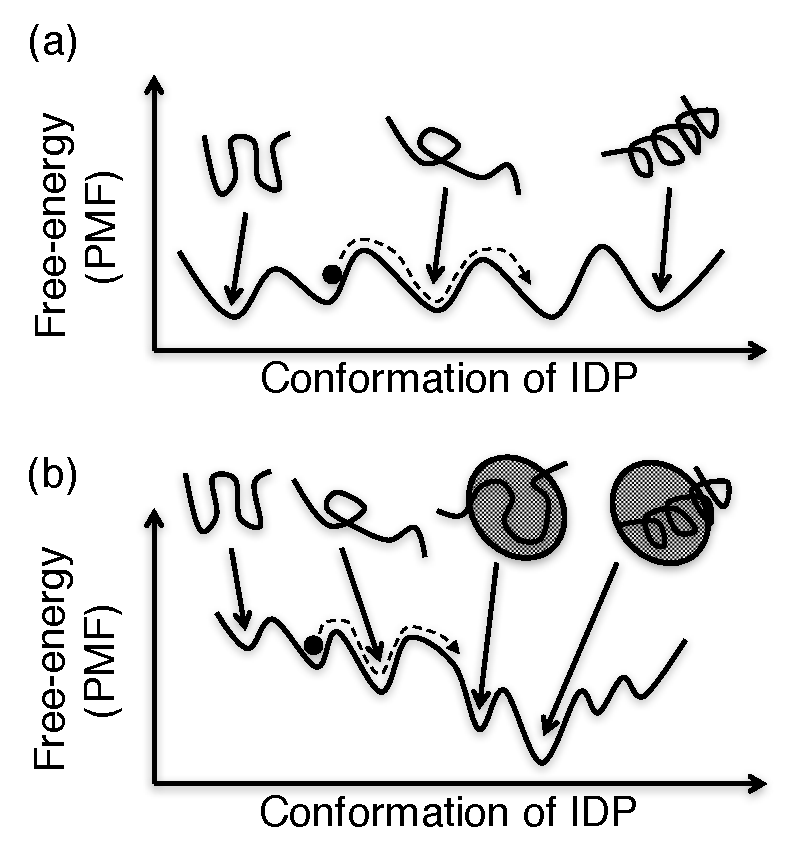
\includegraphics[width=10cm]{../enhance_rev/figures/fel_idps.pdf}
  \caption{\label{fig:fel_idps.pdf} Schematic free-energy landscape of IDP in (a) unbound and (b) bound states shown one-dimensionally. $X$-axis represents conformation of IDP, although the system in panel (b) consists of two molecules (IDP and its partner). Black filled circle represents the IDP conformation moving along simulation trajectory (broken line).}
\end{figure}
An ordered protein has its own tertiary structures (native structure) determined by its aminoacid sequence, and the tertiary structure does not vary largely before and after the complex formation. Contrarily, a unique tertiary structure is not assigned to IDP when the IDP is in the unbound state (isolated state), and the unique structure is formed when it binds to its partner molecules [52-54]. This mechanism is known as “coupled folding and binding” [54]. Therefore, the free-energy landscape of IDP in the unbound state has no dominant cluster prevailing against the other clusters (Figure \ref{fig:fel_idps.pdf}a). In the bound state, contrarily, the landscape has the dominant cluster (the most stable complex) (Figure \ref{fig:fel_idps.pdf}b).

We have computed the free-energy landscape of two systems: NRSF–mSin3 [27] and pKID-KIX [55] systems, where NRSF and pKID are IDPs, and mSin2 and KIX are their partner proteins. In this review, we focus on the NRSF–mSin3 system. NRSF (the N-terminal repressor domain of neural restrictive silencer factor) is an IDP known as an essential transcriptional repressor for neuron-specific genes in non-neuronal cells and neuronal progenitors, and mSin3 is its partner protein. The complex structure was solved by an NMR experiment [56], where a 15-residue segment of NRSF fragment folded into helix when bound to the cleft on the surface of the paired amphipathic helix (PAH) domain of mSin3. The regions of NRSF other than the 15-residue segment are disordered even in the complex structure.

In the McMD simulation, the 15-residue fragment and the PAH domain of mSin3 were treated. We denote the PAH domain of mSin3 simply as mSin3. In the initial conformation of the simulation, these two molecules were distant to each other in an explicit solvent. Furthermore, the conformation of the NRSF segment was disordered in advance (Figure 1c in Ref. 27). After the refinement of multicanonical energy $E_{\rm MC}$ (Eq. \ref{eq:e_mc}) via iterative McMD simulations, production runs were performed yielding the ensemble $Q(300 K)$. McMD of the single NRSF fragment (i.e., unbound state) was also performed with a similar simulation procedure. The initial conformation of the NRSF fragment was randomized in advance and put in an explicit solvent (Figure 1b in Ref. 27).

\begin{figure}
  \centering
  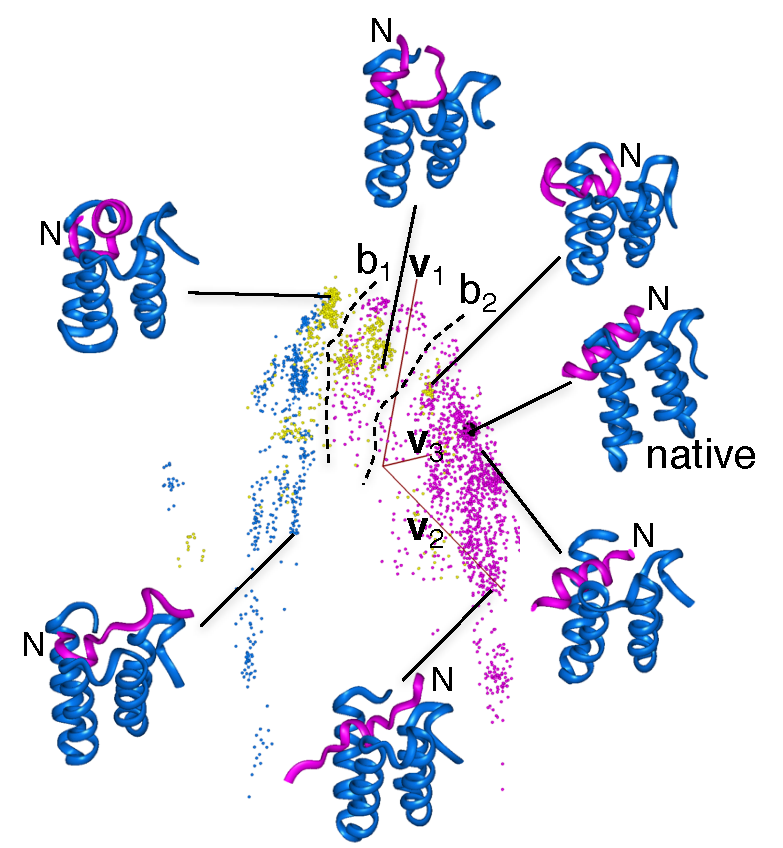
\includegraphics[width=10cm]{../enhance_rev/figures/msin_nrsf_fel.pdf}
  \caption{\label{fig:msin_nrsf_fel.pdf} (a) Conformational distribution of $Q$(300 K) for system consisting of the NRSF fragment and mSin3. The distribution is shown in an abstract thee-dimensional (3D) space, whose coordinate axes (orange-tan colored lines), labeled $\bm{\nu}_1$, $\bm{\nu}_2$ and $\bm{\nu}_3$, are calculated from a principal component analysis (PCA): Each colored dot is projection of a conformation of the NRSF fragment in the 3D space (see Ref. 27). The closer the two dots, the similar the two conformations. Some tertiary structures are also displayed, where magenta model is the NRSF fragment and blue model is mSin3. Yellow spheres indicate the N-terminus of the NRSF fragment. Black sphere represents the position of the NMR complex structure labeled by “native”. There are three large domains spaced by broken lines labeled b1 and b2, along which dots distribute sparsely. Dots are colored depending on mutual molecular orientations between the two molecules: The color is magenta when the NRSF fragment is approximately parallel to the cleft of mSin3, and the color is cyan when they are approximately anti-parallel. Otherwise, the color is yellow. See Ref. 27 for strict coloring method.
}
\end{figure}
Conformational clustering applied to $Q(300 K)$ has shown that the largest cluster (i.e., the most stable cluster) is the native-like complex cluster (Figure \ref{fig:msin_nrsf_fel.pdf} in Ref. 27). Thus, the McMD simulations provided reliable data in the sense that the NMR complex was predicted correctly. In a high-energy range, the NRSF fragment distributed widely in space without a dominant structure (Figure 4A in Ref. 27). Contrarily, at 300 K, the NRSF segment was trapped into the NRSF binding cleft of mSin3 (Figure 4B in Ref. 27). Figure \ref{fig:msin_nrsf_fel.pdf} demonstrates the conformational distribution for $Q(300 K)$ projected in an abstract conformational space. Note that a region with crowded dots (conformations) corresponds to a low free-energy (PMF) region (see Eq. \ref{eq:pmf_gene}). Figure \ref{fig:msin_nrsf_fel.pdf} shows that three domains of crowded dots exist and that the domains were spaced by broken lines labeled b1 and b2, along which the dots distribute sparsely. These sparse-dot regions correspond to free-energy barriers because the probability of conformation around the regions is low. The domains were discriminated well by the molecular orientation of the NRSF fragment in the NRSF binding cleft of mSin3 (see figure legend). Therefore the rearrangement of the molecular orientation of the fragment requires jumping the free-energy barriers. 

\begin{figure}
  \centering
  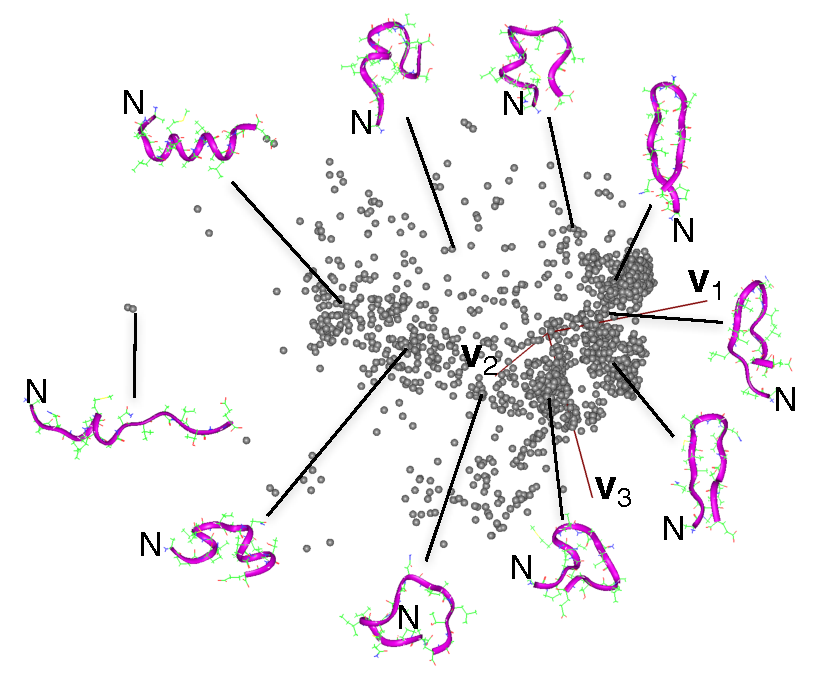
\includegraphics[width=10cm]{../enhance_rev/figures/msin3_fel.pdf}
  \caption{\label{fig:msin3_fel.pdf} Conformational distribution of $Q$(300 K) for single NRSF fragment. Axes $\bm{\nu}_1$, $\bm{\nu}_2$ and $\bm{\nu}_3$ are calculated as with Figure \ref{fig:msin_nrsf_fel.pdf}. Some conformations are also displayed. Yellow spheres indicate the N-terminus of the NRSF fragment.}
\end{figure}
Figure \ref{fig:msin3_fel.pdf} represents the conformational distribution of $Q(300 K)$ for the single NRSF fragment. A variety of conformations, such as helix, hairpin, bent, etc., are seen in the conformational space, which means that the conformation fluctuates among these structures in solution at 300 K: No dominant structure exists. Therefore the NRSF fragment is disordered in the unbound state. Interestingly, most of conformations in  of the single-NRSF system are found in that of the NRSF-mSin3 system, whereas the probabilities assigned to the conformations are different between the two systems (Figure 10 in Ref. 27). The main feature for the complex state was helix, although the single NRSF fragment adopts both the helix and hairpin (Figure 3 in Ref. 27).

From these results, we have proposed a binging mechanism for the coupled folding and binding of NRSF (Figure \ref{fig:msin3_nrsf_regime.pdf}): In the unbound regime, NRSF fluctuates among various conformations. NRSF binds with the cleft of mSin3 with using these conformations, and non-native complexes are formed. The NRSF conformation moves in the bound regime. Otherwise the complex dissociates. Depending on the first formed non-native complex, the complex may overcome one or two free-energy barriers, and finally the native complex is formed. The McMD simulation has shown that the complex formation with the all-atom model is considerably complicated, where the complex experiences various intermediates overcoming free-energy barriers.
\begin{figure}
  \centering
  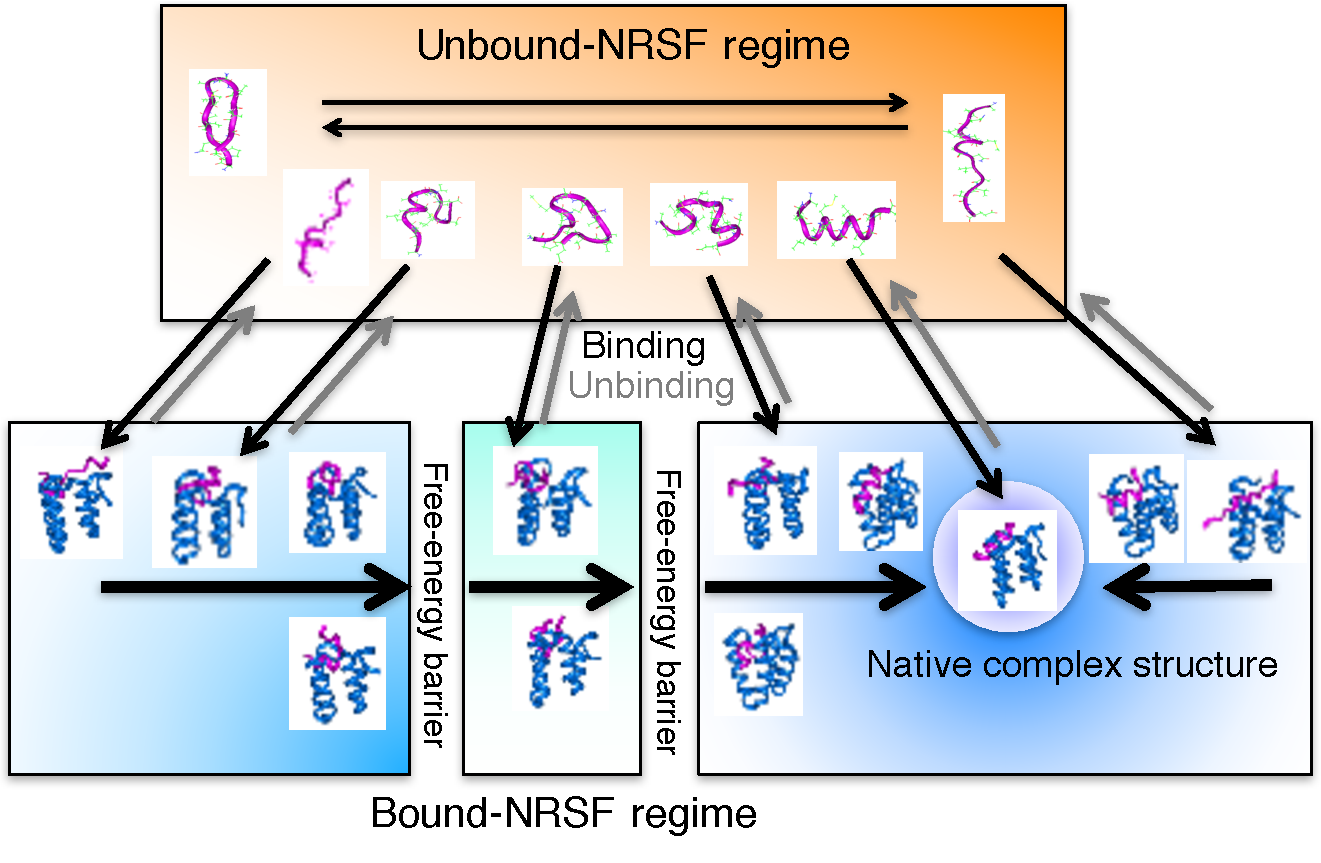
\includegraphics[width=10cm]{../enhance_rev/figures/msin3_nrsf_regime.pdf}
  \caption{\label{fig:msin3_nrsf_regime.pdf} Simplified free-energy landscape integrated from the all-atom detailed free-energy landscapes for the NRSF-mSim3 complex and single-chain NRSF. Arrows represent conformational changes. Yellow spheres in the molecular models indicate the N-terminus of the NRSF fragment.}
\end{figure}

\section{Virtual-system coupling}
Above we have introduced various enhanced conformational sampling methods. Now we introduce a "virtual system", which couples with the biomolecular system (restated as "real system") [57]. The entire system is a sum of the real system and the virtual system, which are specified by the coordinates $\bm{x}$ for the real system (i.e., coordinates of the constituent atoms of the molecular system) and a state parameter for the virtual system. In a simulation, both the real and virtual systems move. Advantageously, one can set the virtual system in an arbitrary manner. We trace the time–development of the entire system instead of pursuing the motions of the real system only. Recently, the virtual-system was integrated with McMD and AUS, which are abbreviated as "V-McMD" [28] and "V-AUS" [58], respectively. Although it may be difficult to understand intuitively the coupling between the real and virtual systems, the computational technique is simple as explained below. See Ref. 28 in detail.

\begin{figure}
  \centering
  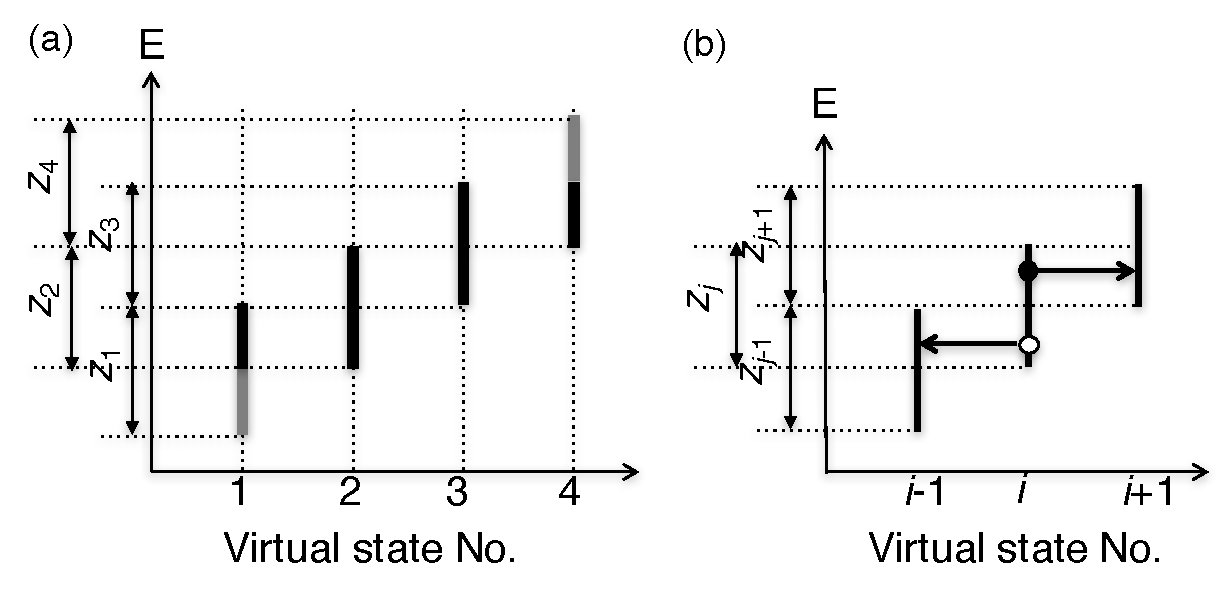
\includegraphics[width=10cm]{../enhance_rev/figures/vstate_transi.pdf}
  \caption{\label{fig:vstate_transi_fig} (a) Space constructed by the energy axis and virtual-state axis, where four virtual states exist as an example. Although the widths of the zones are shown equally in this figure, they are not necessarily the same in the actual sampling. (b) Transitions among adjacent virtual states. See text.}
\end{figure}
Imagine a virtual system, for which the state is specified by a discrete ordinal number  (“virtual-state index”). We assume that when the virtual-state index is $i$, the energy of the real system $E(\bm{x})$ is confined in an energy zone $z_i$ as: $z_i = [E^{\rm min} \leq E_i  \leq E^{\rm max}]$. Figure \ref{fig:vstate_transi_fig}a represents a space constructed by the energy axis and virtual-state axis. Zones $z_{i-1}$ and $z_i$ ($z_1$ and $z_2$ for instance) overlap to each other as well as $z_i$ and $z_{i+1}$ ($z_2$ and $z_3$ for instance) do, although two zones $z_{i-1}$ and $z_{i+1}$ do not overlap because the zones are set as: $[E^{\rm min}_{i+1} - E^{\rm max}_{i-1}] > \epsilon$, where $\epsilon$ is a positive but an infinitely small number. In time-development of the entire system, the conformation of the real system varies according to the equations of motion, and the virtual-state index jumps from $v_i$ to $v_{i+1}$ or $i-1$, by which the variable energy range for the real system is reset. If inter-virtual state transitions are exhibited in the simulation, the real system fluctuates within $z_i$, which means that only a narrow region of the conformational space is sampled (i.e., sampling efficiency is low). We define the inter-virtual state transitions as follows: Suppose that $E$ is at the filled-circle position in Figure \ref{fig:vstate_transi_fig}b. Then the virtual state $i$ may jump to the virtual state $i+1$ without changing $\bm{x}$ of the real system. On the other hand, if $E$ is at the open-circle position, the virtual state may transition to $i-1$. Then, we introduce a rule: during a time interval of $[t,t+\tau]$, the virtual state number is fixed to $i$, and $\bm{x}$ moves according to the ordinary equations of motion with confining $E$ in $z_i$. At time $t+\tau$ the transition is achieved to $z_{i-1}$ or $z_{i+1}$ with the transition probability  $\rho_t$ ($0 \leq \rho_t \leq 1$), at which $\bm{x}$ does not move. Due to the arbitrary property of the virtual system, one can set arbitrarily the transition probability $\rho_t$ and the interval $\tau$, which may increase the sampling efficiency [28,57]. Consequently, with traveling the virtual states, the real system fluctuates the wide conformational space overcoming energy barriers. The detailed balance for this time–development is theoretically well satisfied as described in APPENDICES. Introduction of the virtual system to AUS is explained in Ref. 58. 

Recently, Moritsugu et al. introduced “multiscale essential sampling (MSES)”, where a protein system was expressed by an all-atom model, and coupled with a coarse-grained (CG) model(s) to enhance conformational sampling [59,60]. MSES was applied to protein-protein binding of a barnase-barstar system [61]. The free-energy landscape for association/dissociation demonstrated existence of the non-native complex forms as well as the native-complex. Although the methodological fashion of MSES is considerably different from the virtual-system coupling method, the two methods have a similarity in the introduction of non-realistic systems to be coupled with the real system.

\section{A free energy landscape for dimer formation by V-McMD \label{et1_sec}}
Here, as an example of generalized ensemble method applied to a biomolecular complex formation, we show the free-energy landscape of homo-dimer formation of an endothelin-1 (ET1) derivative computed by V-McMD simulations. ET1 is a biomolecule of 21 aminoacids long known as a strong vasoconstrictor on smooth muscles of a vessel [62-64]. This molecule is a potent drug target because it is related to many human diseases [65-69]. The tertiary structure was solved by NMR spectroscopy [70-72] and X-ray crystallography [73]. In either study, the N-terminal region adopts a strand and the middle region forms an $\alpha$-helix. Because two disulfide bonds link the strand and the helix, the tertiary structure is compact and stable regardless of its short polypeptide length. 

\begin{figure}
  \centering
  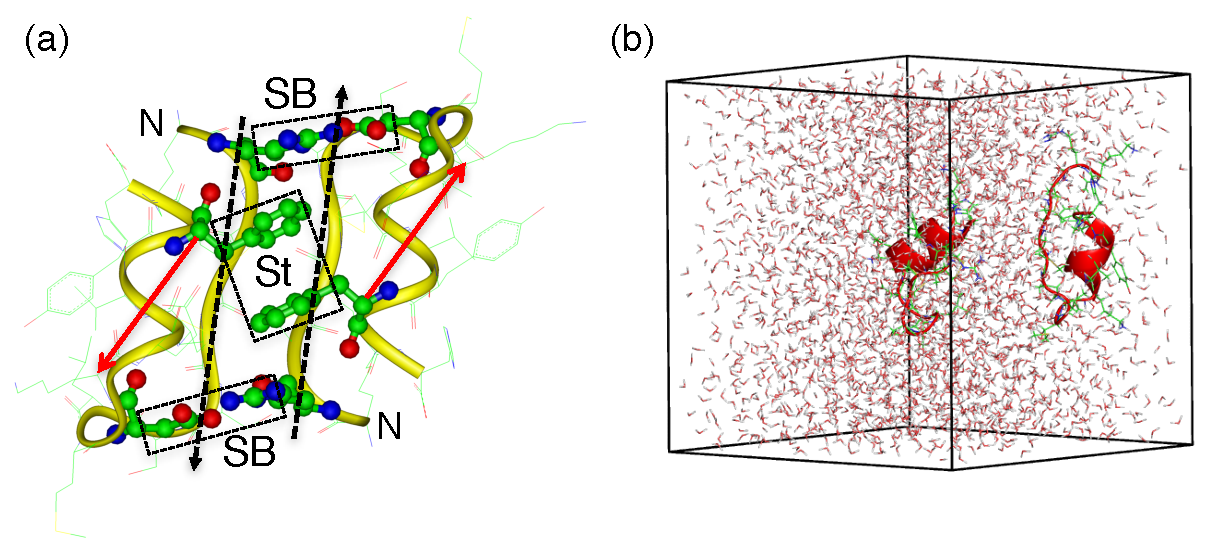
\includegraphics[width=10cm]{../enhance_rev/figures/et1_conf.pdf}
  \caption{\label{fig:et1_conf_fig} Homo-dimer complex of KR-CSH-ET1 determined by X-ray crystallography. Two “N” characters indicate the N-termini of the molecules. Inter-molecular $\beta$-sheet is formed between two strands indicated by black broken-line arrows. Inter-molecular hydrophobic stacking between phenylalanine side-chain rings is shown by the rectangle labeled “St”. Two inter-molecular salt bridges, formed between arginine and aspartic acid, are indicated by the rectangles labeled “SB”. Red arrows are used for identifying the molecular orientations of the two molecules, which point from the C$\alpha$ atom of Lys to the C$\alpha$ atom of the last Cys in the sequence of KR-CSH-ET1. (b) Initial conformation of V-McMD simulation.}
\end{figure}
ET1 aggregates at concentration of 1-4 mM. Then, to increase the solubility the N-terminal was extended by two charged aminoacid residues, Lys and Arg [74], which exist in its precursor protein. This extended ET1 is denoted as KR-ET1. Unexpectedly and interestingly, KR-ET1 has less activity than ET1 does in spite of increment of solubility. Then, an X-ray crystallography [75] showed that KR-ET1 forms a homo-dimer (PDBID; 1t7h) (Figure \ref{fig:et1_conf_fig}a), where the orientations of the two molecules are anti-parallel to each other although its molecular tertiary structure is similar with the single ET1 structure. In the study, five aminoacid residues at the C-terminal of KR-ET1 were removed because those residues are presumably disordered and exposed in solution. This truncated peptide of 18 aminoacids long (sequence: KRCSCSSLMDKECVYFCH) is denoted as KR-CSH-ET1. Figure \ref{fig:et1_conf_fig}a indicates that this complex is stabilized by three factors: inter-molecular $\beta$-sheet, inter-molecular hydrophobic stacking of phenylalanine side-chain rings, and two inter-molecular salt bridges. Therefore, the experimental study of Ref. 75 reported that this homo-dimer structure is considerably stable.

The dimer formation of KR-CSH-ET1 is an appropriate target for assessing V-McMD because the complex form is discriminated well by two quantities: the mutual molecular orientation $\bm{e}_{a1} \cdot \bm{e}_{a2}$ and the inter-molecular separation distance $r_{12}$, whose exact definition is given later. Previously we performed V-McMD simulations for KR-CSH-ET1 dimer formation [28], where the two molecules were confined in a spherical droplet of an explicit solvent, and the two-dimensional free-energy landscape was computed. The free-energy landscape at room temperature was predominantly composed of the crystallographic native complex structure. In the current review, we performed V-McMD of KR-CSH-ET1 dimer formation with periodic boundary condition, and computed the free-energy landscape. 

The simulation system was generated as follows: One KR-CSH-ET1 was immersed at the center of a periodic box (box size:  $45.000^3 \AA^3$) filled by an explicit solvent, and the other KR-CSH-ET1 was put at a position apart from the first KR-CSH-ET1 molecule. The system consisted of 8706 atoms (580 atoms for the KR-CSH-ET1 molecules, 9 Na+, 11 Cl- ions, and 2702 water molecules). The number of ions was determined to set the solution at a physiological salt concentration. Then a constant-pressure MD simulation (i.e., NPT simulation) was performed at room temperature and pressure of 1.0 atm, by which the initial conformation for V-McMD was prepared (resultant box size: $44.004^3 \AA^3$) (Figure \ref{fig:et1_conf_fig}b). The V-McMD simulation procedure was similar with that for the previous study [28] as follows: First refinement of $E_{\rm MC}$ was done via iterative V-McMD simulations, and then the production V-McMD simulation was performed to produce an entire conformational ensemble. The conformational ensemble $Q(T_{\rm room})$ was constructed by reweighting the snapshots in the entire ensemble. 

In V-McMD the energy moves in a wide range as mentioned previously. Then, KR-CSH-ET1 may unfold when the system is elevated to a high-energy region. The purpose of the current study is to show the free-energy landscape for the molecular binding, and refolding of KR-CSH-ET1 is outside the scope. Thus, we restrained weakly the tertiary structure of each KR-CSH-ET1 by intra-molecular restraint functions (see Ref. 28 for technical details). Thus, translational and rotational motions of the KR-CSH-ET1 molecules were free with maintaining their tertiary structures.

In this study, we set $T_{\rm room}$=300 K and obtained a canonical ensemble . Figure 12a demonstrates a free-energy landscape at 310 K presented two-dimensionally by $\bm{e}_{a1} \cdot \bm{e}_{a2}$ and $r_{12}$, whose exact definition is given in the figure legend. From this figure, the largest cluster (i.e., the lowest free-energy cluster) is native-like, where the two KR-CSH-ET1 molecules are arranged in anti-parallel, and the three factors, mentioned above, stabilized the complex structure. We call this cluster the native-like cluster. The landscape provided two other clusters. In the second largest cluster (the second lowest free-energy cluster), the orientations of the two KR-CSH-ET1 molecules are perpendicular to each other approximately: $\bm{e}_{a1} \cdot \bm{e}_{a2} \approx 0$. The third largest cluster (the third lowest free-energy cluster) was characterized by $\bm{e}_{a1} \cdot \bm{e}_{a2} \approx 1$, which means that the relative orientations of the two molecules are parallel. In the solvent-droplet boundary condition [28], the free-energy landscape had only the native-like cluster. It is likely that the solvent-droplet boundary condition would result in a stronger pressure than 1 atm in the droplet center due to the surface tension of the spherical droplet. This strong pressure could stabilize the well-packed conformation (i.e., native complex), and then probabilities assigned to the non-native complexes were diminished. The periodic boundary condition does not induce such an artificial excess pressure because there is no free surface in this treatment.

\begin{figure}
  \centering
  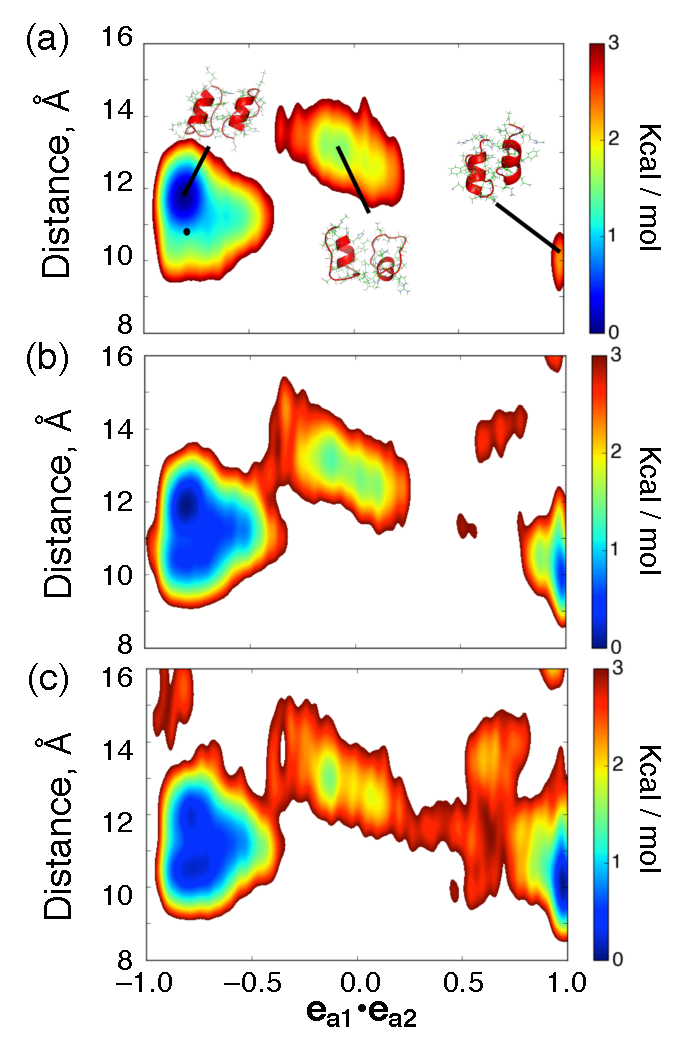
\includegraphics[width=10cm]{../enhance_rev/figures/dimer_form_fel.pdf}
  \caption{ \label{fig:dimer_form_fel_fig} 
Free-energy landscapes at (a) 310 K, (b) 350 K, and (c) 370 K. X-axis is mutual molecular orientation $\bm{e}_{a1} \cdot \bm{e}_{a2}$, where $\bm{e}_{a1}$ and $\bm{e}_{a2}$ are unit vectors parallel to the red-colored vectors in defined in Figure \ref{fig:et1_conf_fig}a: $-1 \leq \bm{e}_{a1} \cdot \bm{e}_{a2} \leq1$. Orientations of two KR-CSH-ET1 molecules are approximately parallel, anti-parallel, and perpendicular to each other for $\bm{e}_{a1} \cdot \bm{e}_{a2} \approx 1$, $\bm{e}_{a1} \cdot \bm{e}_{a2} \approx -1$, and $\bm{e}_{a1} \cdot \bm{e}_{a2} \approx 0$, respectively. Y-axis is inter-molecular separation distance $r_{12}=|\bm{r}_{G1}-\bm{r}_{G2}|$, where $\bm{r}_{G1}$ and $\bm{r}_{G2}$ are positions of the geometrical centres of the two molecules, and the geometrical centre is computed from the C$\alpha$-atomic positions of each molecule. The free-energy value (PMF; Eq. 1), whose height is shown by the coloured scale bars, is set so that the lowest PMF is zero. Tertiary structures from three clusters at 300 K are shown in panel (a), where the small black filled circle indicates the position of the native complex experimentally determined.}
\end{figure}

Figures \ref{fig:dimer_form_fel_fig}b and c demonstrate free-energy landscapes at 350 K and 370 K, respectively. The largest and second largest clusters are connected at 350 K, although the third largest cluster is still isolated. At 370 K, the third largest cluster is connected to the second largest cluster. We presume that once a non-native complex is formed in the cluster of $\bm{e}_{a1} \cdot \bm{e}_{a2} \approx 0$ , this complex can transition to the native-like cluster relatively readily. Contrarily, once a non-native complex is formed in the cluster of $\bm{e}_{a1} \cdot \bm{e}_{a2} \approx 1$, this complex should overcome a high-energy barrier to reach the native-like cluster via the cluster of $\bm{e}_{a1} \cdot \bm{e}_{a2} \approx 0$ . Otherwise, this complex dissociates, and the free KR-CSH-ET1 molecules may re-associate after that. Another interesting result from Figure \ref{fig:dimer_form_fel_fig} is that the second largest cluster at 300 K and 350 K is the third largest cluster at 370 K.

We exemplify in this section that the generalized ensemble method is a powerful tool to compute the free-energy landscape, by which we can discuss the thermodynamic stability of the clusters, the cluster networks, and the temperature dependence of the networks.

\section{Concluding remarks}
In this review, we introduced various generalized ensemble methods especially focusing on methods applicable to biomolecular association/dissociation with an atomistic resolution in explicit solvent to obtain the free-energy landscape. For making the methods useful for drug-discovery, the methods should not only explain basic mechanisms for association/dissociation, but also predict the complex forms and their stabilities. From this point of view, the sampling methods are useful if they generate a free-energy landscape for complex formation in explicit solvent at the atomistic resolution. In the introduction-section, we listed three approaches: fast computations, multiple simulation runs, and generalized ensemble methods. Note that these approaches can be combined. For instance, trajectory parallelization has been used for multicanonical and adaptive umbrella sampling. The free-energy landscape obtained from the generalized ensemble method does not involve information on rate constants. However, from the knowledge about the locations of many locally stable states, it is possible to look for the shortest path between a pair of conformational clusters, for example, by the string method [76], and the activation energy overcoming the energy barrier can be computed. In addition, combination of the generalized ensemble methods with the rate-constant estimation method using the Markov state model [7,8] among conformational clusters may be useful. 

In living matter, a number of biological molecules (proteins, metabolites, and DNAs) are crowding in solution (water and ions). Recent studies are revealing that crowding itself provides and/or enhances activities of the biomolecules [77, 78]. These large-scale studies, however, view the biomolecules neglecting their atomic details. Therefore, detailed intermolecular information from the generalized ensemble methods is useful to complete the molecular picture for living matter. 

Most of MD simulations currently used are based on the classical mechanics (Newtonian dynamics). On the other hands, many important processes taking place in living matter, such as catalytic reactions, are quantum chemical. Thus, development of quantum-mechanical molecular dynamics [79-83] is an important step to elucidate vividly biochemical reactions in living matter, whereas there is a distance to be applied to large biomolecular systems. One of the goals of the generalized ensemble methods is to be coupled with the quantum-mechanical technique in the molecular crowding environment.
